% Official MDPI class, Mathematics, submission layout. XeLaTeX/Tectonic: no pdftex option.
\documentclass[mathematics,article,submit,moreauthors]{Definitions/mdpi}
\firstpage{1}
\pubvolume{1}
\issuenum{1}
\articlenumber{0}
\pubyear{2026}
\copyrightyear{2026}
\datereceived{ }
\daterevised{ }
\dateaccepted{ }
\datepublished{ }
\doinum{}
\hreflink{DOI not assigned}
\providecommand{\norm}[1]{\left\lVert#1\right\rVert}
\emergencystretch=3em
\setlength{\headheight}{24pt}
% Keep the official class unmodified. Tectonic cannot directly include its EPS logos.
% build_paper_submission.py makes vector PDF copies with Ghostscript.
\let\OriginalIncludeGraphics\includegraphics
\renewcommand{\includegraphics}[2][]{%
  \IfStrEq{#2}{Definitions/logo-mdpi.eps}
    {\OriginalIncludeGraphics[#1]{converted/logo-mdpi.pdf}}
    {\IfStrEq{#2}{Definitions/logo-updates.eps}
      {\OriginalIncludeGraphics[#1]{converted/logo-updates.pdf}}
      {\OriginalIncludeGraphics[#1]{#2}}}}
\fancypagestyle{plain}{%
  \fancyhf{}%
  \fancyfoot[L]{\footnotesize Working draft for author review}%
  \fancyfoot[R]{\footnotesize Not submitted; DOI not assigned}%
  \renewcommand{\headrulewidth}{0pt}%
  \renewcommand{\footrulewidth}{0.4pt}}
\lhead{\fontsize{8}{8}\selectfont Working draft for \emph{Mathematics}; not submitted\\
\rule{\fulllength}{0.4pt}}
% Automatic table width: fill textwidth; use the MDPI full-page span only if needed.
% Keep generated table data untouched. Measure at the table's own font size.
\usepackage{xparse}
\newsavebox{\PaperTableMeasureBox}
\newdimen\PaperTableNaturalWidth
\newdimen\PaperTableTargetWidth
\let\PaperOriginalTable\table
\let\PaperOriginalEndTable\endtable
\let\PaperOriginalTabular\tabular
\let\PaperOriginalEndTabular\endtabular
\RenewDocumentEnvironment{table}{O{H}+b}{%
  \global\PaperTableNaturalWidth=0pt
  \begingroup
    \renewcommand{\caption}[2][]{}
    \renewcommand{\label}[1]{}
    \RenewDocumentEnvironment{tabular}{O{c}m+b}{%
      \sbox{\PaperTableMeasureBox}{\PaperOriginalTabular[##1]{##2}##3\PaperOriginalEndTabular}%
      \ifdim\wd\PaperTableMeasureBox>\PaperTableNaturalWidth
        \global\PaperTableNaturalWidth=\wd\PaperTableMeasureBox
      \fi
    }{}%
    \setbox0=\vbox{\hsize=\fulllength\linewidth=\fulllength #2}%
  \endgroup
  \begingroup
  \PaperOriginalTable[#1]
  \PaperTableTargetWidth=\textwidth
  \ifdim\PaperTableNaturalWidth>\textwidth
    \PaperTableTargetWidth=\fulllength
  \fi
  \typeout{PAPER-TABLE natural=\the\PaperTableNaturalWidth; target=\the\PaperTableTargetWidth}%
  \RenewDocumentEnvironment{tabular}{O{c}m+b}{%
    \ifdim\PaperTableNaturalWidth>\PaperTableTargetWidth
      \PackageWarning{paper-tables}{Table exceeds full width; scaling to fit}%
      \resizebox{\PaperTableTargetWidth}{!}{%
        \PaperOriginalTabular[##1]{##2}##3\PaperOriginalEndTabular}%
    \else
      \begin{tabular*}{\PaperTableTargetWidth}[##1]{@{\extracolsep{\fill}}##2}%
        ##3
      \end{tabular*}%
    \fi
  }{}%
  \ifdim\PaperTableTargetWidth>\textwidth
    \begin{adjustwidth}{-\extralength}{0cm}
      \captionsetup{width=\PaperTableTargetWidth}%
      #2
    \end{adjustwidth}
  \else
    \captionsetup{width=\PaperTableTargetWidth}%
    #2
  \fi
  \endtable
  \endgroup
}{}
% Generated; do not hand edit.
\newcommand{\FinalNative}{0.1869}
\newcommand{\FinalDense}{0.1837}
\newcommand{\FinalMidas}{0.1849}

\Title{SOKKANAEM: Change-Gated State-Space Modeling with Cached Readout for Streaming Video Depth}
\TitleCitation{SOKKANAEM for Streaming Video Depth}
% The user will supply these details. Do not submit with placeholders.
\Author{Author information to be completed}
\AuthorNames{Author information to be completed}
\AuthorCitation{Author information to be completed}
\address{Affiliation and institutional address to be completed by the author.}
\corres{Correspondence: to be completed by the author.}

\abstract{Streaming video depth requires dense predictions on every frame, even when much of the image changes little. We present SOKKANAEM, a 4.19-million-parameter recurrent model that combines patch-change gating, selective state-space updates, temporal and spatial output caches, and a dense depth decoder. Binary gating preserves inactive temporal states, while periodic refresh and an all-active fallback limit reuse duration and handle high activity. We evaluate the frozen model with same-weight controls that separate state carry, retained-state readout, spatial context and output reuse. On four reserved TUM sequences, the reference model obtains clip scale--shift AbsRel \FinalNative{} at 256 frames, compared with \FinalDense{} for dense carry and \FinalMidas{} for MiDaS Small. Its motion-referenced TCE is 0.0352 versus 0.0640 for MiDaS, although its scale variation is not uniformly smaller. The measured development PNG-to-depth latency is 7.496 ms/frame versus 7.521 for dense carry. Thus, computational reuse does not yet establish substantial pipeline acceleration. Conditional error and cache-age analysis explains the design trade-offs. The contribution is a compact streaming architecture and a controlled characterization of its accuracy, temporal behavior and implementation cost, rather than a claim of universal performance superiority.}
\keyword{state-space model; conditional computation; video depth; error propagation; cache refresh; reproducible evaluation}

\begin{document}

\section{Introduction}
Video depth estimation supplies a dense geometric signal for each arriving RGB frame.
Processing every frame independently discards temporal information and repeatedly evaluates
similar regions. A streaming model should instead reuse useful history while maintaining
depth quality, responding to scene changes and controlling per-frame execution cost.

We present SOKKANAEM, a compact recurrent video-depth architecture built around
patch-level visual change. An external, untrained detector selects temporal state updates;
separate temporal and spatial caches reuse block outputs; a dense decoder still predicts
depth at every pixel. The input is the current frame and a stream-specific state dictionary,
so the native prediction path does not require future frames, optical flow or ground truth.
Fixed-period refresh and a high-activity fallback complement the change gate.

The central design question is how to combine temporal memory and computational reuse
without confusing a held internal state with an unchanged or accurate output. Our model
exposes state carry, readout reuse, spatial caching and refresh as distinct mechanisms.
This makes their effects testable with the same trained weights rather than attributing
every difference to a single sparsity score.

Our contributions are (i) a 4.19M-parameter streaming architecture combining externally
gated selective SSMs with cached readout and dense depth prediction; (ii) same-weight,
matched-mask interventions identifying the roles of retained-state readout and spatial
context; (iii) evaluation of aligned accuracy, motion-referenced temporal error, scale
variation and input-to-output cost; and (iv) conditional design analysis of state error,
cache age and refresh overhead. The existing perturbation inequalities support the
architecture's design rationale; they are not presented as new universal stability laws.

The frozen reference does not dominate all controls or baselines. In particular,
its measured desktop pipeline latency is close to dense carry, and lower short-step
variation does not imply lower long-clip scale variation. We distinguish these observed
trade-offs from the design objective of faster, temporally reliable streaming inference.

\section{Related Work}
Skip RNN explicitly uses a binary update/copy operation~\cite{campos2018}. Mamba introduces
input-selective state-space dynamics and hardware-aware scanning~\cite{gu2024}. We do not
claim either binary preservation or input selection as a first contribution.
DeltaCNN propagates sparse frame differences through CNN operators~\cite{deltacnn}, and
Eventful Transformers reuse computation based on changing tokens~\cite{eventful}.
Change-based reuse itself is therefore also established. Spiking SSMs such as
SPikE-SSM~\cite{spikessm} and SpikySpace~\cite{spikyspace} investigate sparse dynamics
in sequence learning and forecasting. Their architectures and tasks differ from dense
RGB video-depth readout, but they preclude a broad claim of the first sparse or event-driven SSM.

The distinction investigated here is the combination of externally selected patch updates,
selective SSM states, separate output caches, and measured depth/pipeline error.
The literature comparison is targeted, not an exhaustive priority search. We do not report
cross-task numerical comparisons against those methods. DPT~\cite{dpt}, MiDaS~\cite{midas}
and Depth Anything V2~\cite{da2} provide independent-image depth references, not a complete
benchmark of causal and noncausal video-depth systems.
Video Depth Anything (VDA)~\cite{vda} adds a spatial--temporal depth head;
online VDA~\cite{ovda} is a distinct online formulation. Historical VDA scores in
this repository do not have frame-ID and weight/source-hash linkage sufficient
for inclusion in the frozen comparison. The audited historical wrapper calls
a 32-frame offline, unmasked temporal-attention path, not frame-causal inference.
The supplementary audit preserves those results separately. A matched modern
video-depth baseline remains a limitation, not a completed comparison.

\section{SOKKANAEM: A Change-Gated Streaming Depth Model}
\subsection{Architecture and reference configuration}
The model uses a stride-16 RGB embedding, four alternating temporal/spatial blocks,
192-dimensional tokens, inner dimension 384, state dimension 16, four-direction spatial
scans, local spatial convolution, and a dense DPT-style binned depth decoder.
It has 4,185,872 parameters. The baseline is the seed-0 EMA checkpoint at 256 pixels,
with pixel-MSE hysteresis thresholds 0.05/0.025, keyframe interval 30, both output caches,
and an all-active fallback above activity 0.4. GMC is disabled in the primary model.
The recorded training ancestry contains 60k, 60k, 25k and 8k stage steps; this is not an
independently verified optimizer-update count or evidence of teacher-free ancestry.
\begin{figure}[H]
\begin{adjustwidth}{-\extralength}{0cm}
\centering
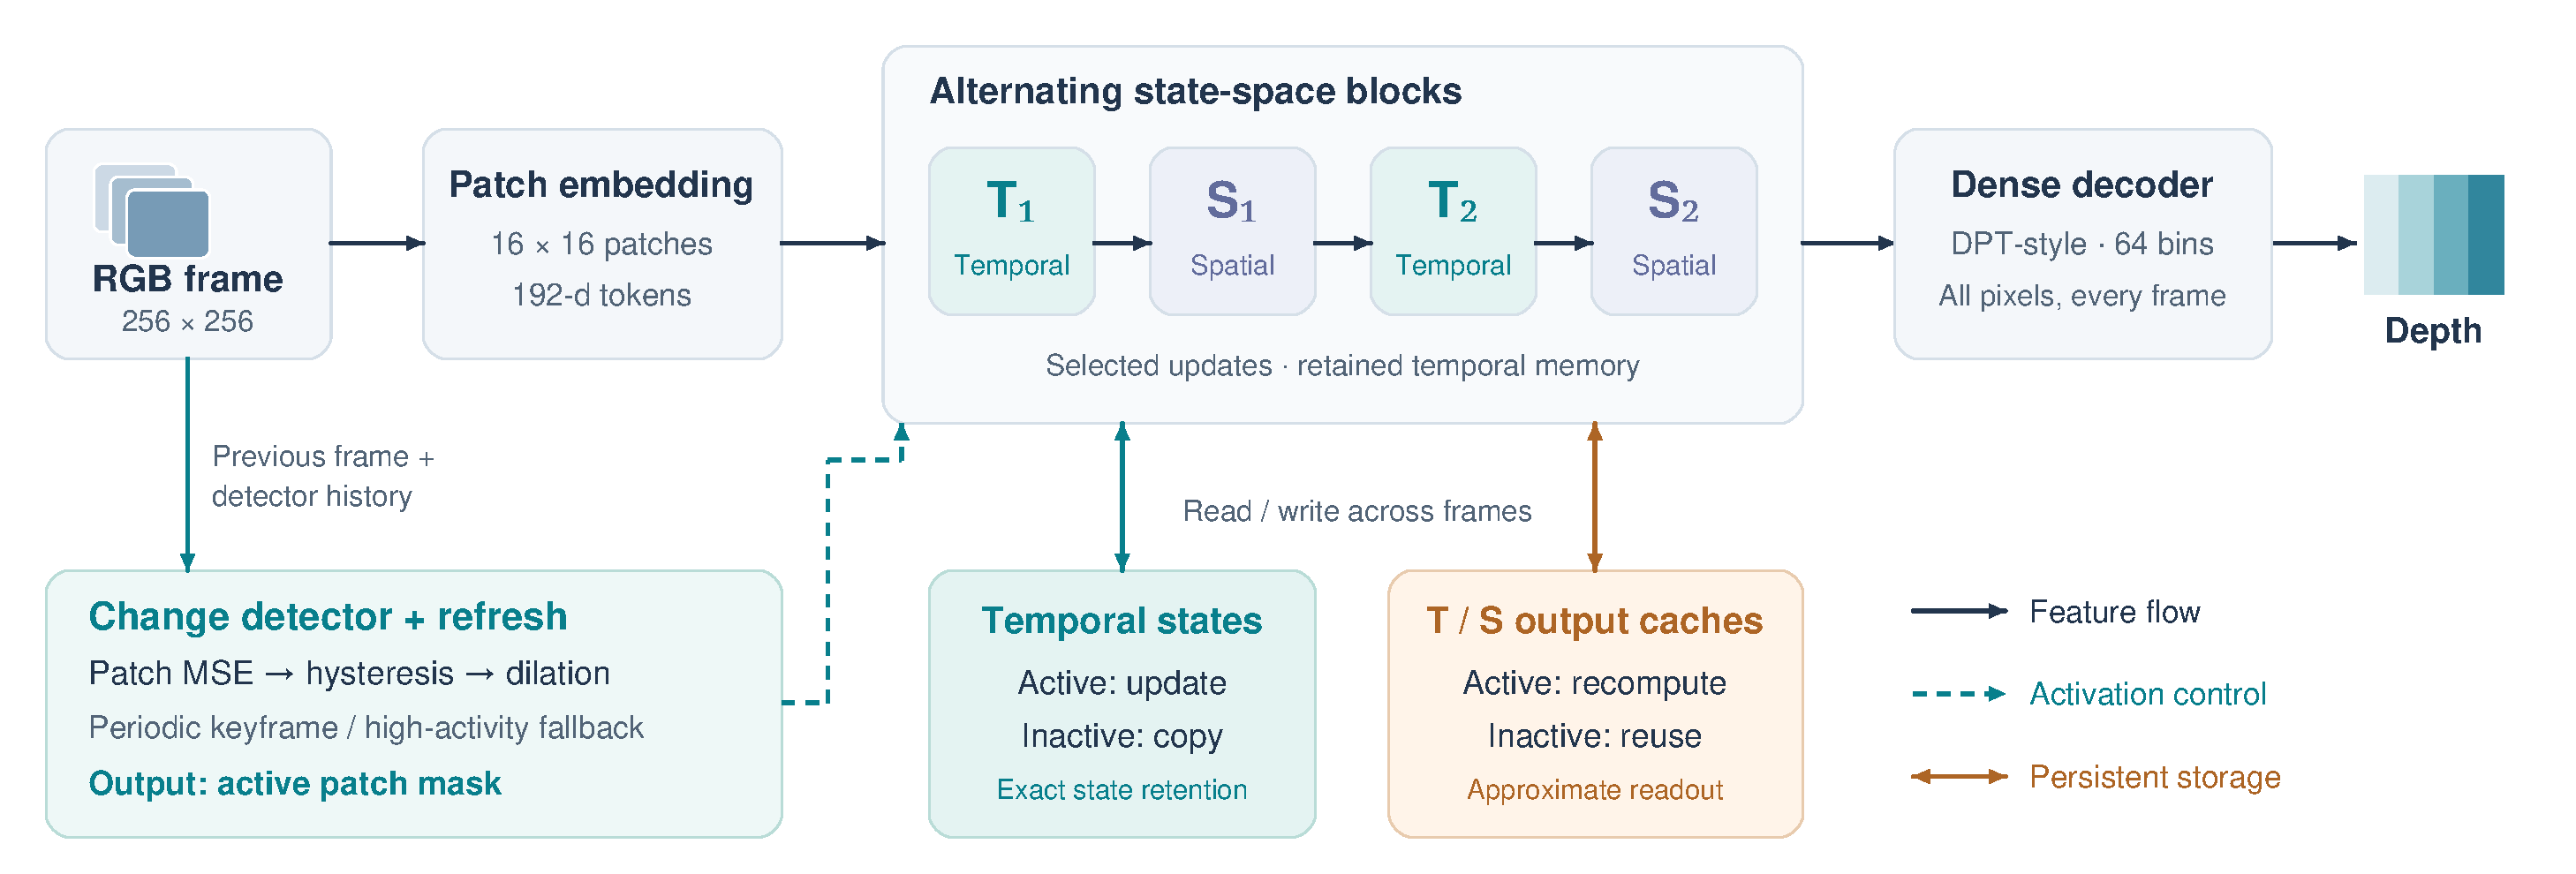
\includegraphics[width=\fulllength]{figures/r3_architecture.pdf}
\caption{SOKKANAEM architecture. The upper path maps each RGB frame through
patch embedding, four alternating temporal (T) and spatial (S) state-space blocks,
and a dense depth decoder. The change detector supplies the activation mask
(dashed arrows); bidirectional arrows denote access to persistent temporal states
and T/S output caches across frames. Inactive temporal states are copied exactly,
whereas cached readout and omitted spatial context introduce approximations.
The depth icon is illustrative, not a measured prediction. Arrows show conceptual
data/control flow rather than kernel execution order.}\label{fig:architecture}
\end{adjustwidth}
\end{figure}

\subsection{Change selection and refresh}
For patch $i$ with $Cp^2$ RGB values, the detector computes
\[
 d_{t,i}=\frac{1}{Cp^2}\sum_{u\in i}(I_t(u)-I_{t-1}(u))^2.
\]
It uses threshold $\tau_{\rm off}$ for a previously active detector patch and
$\tau_{\rm on}$ otherwise, followed by one-patch dilation. The first frame and
frames whose zero-based index is divisible by $K$ activate every patch.
At batch one, the model additionally switches to all-active execution if the
detector mask's mean activity exceeds 0.4. Detector hysteresis bookkeeping and
the model's post-detector fallback are distinct; fallback does not rewrite the
stored detector mask. These rules are fixed heuristics, not learned uncertainty
estimates or an adaptive error certificate.

\subsection{Temporal memory, cached readout and spatial context}
Each temporal block maintains a hidden state for every patch. Without temporal
output caching, an inactive hidden state is preserved but the block can still
read it using current-input-dependent parameters. With temporal caching enabled,
inactive block outputs are reused and the corresponding temporal computation
is bypassed. These two modes separate state preservation from readout reuse.

Spatial blocks use four-direction scans and local spatial convolution. The
spatial-cache path processes a selected token subsequence and restores dense
block outputs by combining updates with cached entries. Omitting inactive
spatial context can affect active tokens as well; this path is an approximation,
not dense-network equivalence. The decoder fuses intermediate block features
with RGB information and emits a full depth map at every step. Sparse backbone
updates therefore do not make the embedding or decoder free.

\subsection{Streaming execution and training}
A stream starts with empty temporal states and caches. For each arriving frame,
the model (1) selects the detector mask and applies any forced full update,
(2) embeds the frame, (3) traverses temporal and spatial blocks with the selected
state/cache policies, (4) decodes dense depth, and (5) returns the updated stream
state. Separate state dictionaries allow interleaved streams to share weights.
Neither the predictor nor its change detector consumes the evaluation GT or RAFT flow.

We evaluate the existing v11 seed-0 EMA checkpoint, not a newly trained variant.
Its recorded final stage uses 8000 steps, length-24 clips, batch two, random masks
with maximum skip fraction 0.5 and the recorded depth/gradient/normal/bin/warp/edge/spread
loss settings. The training mask is not the deployment change detector, leaving
a train--deploy mismatch. Full settings and ancestry limitations are in the
reproduction appendix. No adaptive-refresh policy or improved encoder/decoder
is claimed to have been trained or evaluated in this revision.

\section{Design Rationale and Conditional Guarantees}

\subsection{State preservation and approximation}
For a shared token input, write $F_t(h)=\Phi_t h+q_t$, with
$\Phi_t=\operatorname{diag}(\exp(-\lambda_j\Delta_{t,j}))$ and
$q_{t,j}=\Delta_{t,j}(B_tx_t)_j$. Binary gating implements
$\widetilde h_t=M_tF_t(\widetilde h_{t-1})+(I-M_t)\widetilde h_{t-1}$.
Zero step preserves state, but the input term is a first-order approximation to exact
ZOH. Current-input-dependent readout and spatial-context omission need separate analysis.

With $e_t=\widetilde h_t-h_t$ and
$r_t=(I-M_t)((I-\Phi_t)\widetilde h_{t-1}-q_t)$, the exact shared-input identity is
$e_t=\Phi_te_{t-1}+r_t$. Products of transition norms bound the propagated initial
error and injected defects. A uniform geometric bound additionally requires a uniform
contraction and a valid defect bound. Different deep-layer token trajectories add
parameter/input perturbations; a negative diagonal $A$ alone does not certify the full network.

The first temporal block admits a conditional cache bound
$L_R\norm{W}a\sqrt{Cp^2\tau_{\rm on}}$ after $a$ inactive steps, provided the
state-fixed readout has the stipulated Lipschitz constant. It is not a tau-only
depth guarantee. Keyframes bound cache age by $K-1$ and remove the local approximation
at the same incoming state, but they do not recover the state of a continuously dense history.
Full assumptions, proofs, counterexamples and the no-fit AbsRel connection are in Appendix~\ref{app:proofs}.

\subsection{Paid computation}
Under the explicitly additive model $C_d=F+V$ and
$\overline C_s=F+\overline a_{\rm eff}V+\overline H$, normalized speedup is
$[f+(1-f)\overline a_{\rm eff}+\omega]^{-1}$. Overhead must be smaller than
saved variable cost for acceleration. This is Amdahl-style reasoning~\cite{amdahl1967},
not a conversion of MAC reductions into observed time. Keyframes and fallback events
are counted as a union. At 256 frames and $K=30$, even a static stream has nine keyframes.
The analysis links two constraints on refresh: a certified cache-only tolerance
would impose an upper bound on $K$, whereas a target speedup in the fixed-cost
model imposes a lower bound. Their intersection is a conditional design check,
not a selected operating point or an accuracy certificate. The constants needed
for a useful numerical cache guarantee have not been certified for this network.

\section{Experimental Setup}
\subsection{Development and reserved transfer sequences}
The previously reused TUM/Bonn holdout is development data, not an independent test.
It contains 488 L8 clips, of which 487 have scorable GT, and 13 L256 clips (3328 frames)
from four sequences. The final evaluation uses four reserved TUM Freiburg3 sequences:
sitting\_xyz, sitting\_rpy, walking\_xyz and walking\_rpy. The frozen lists contain
462 L8 clips and 13 L256 clips. These are new sequences in the same capture setting;
they do not establish scene-disjoint or fixed-camera generalization. L32 is not evaluated
in this final protocol. The lengths share underlying footage and are not independent samples.
RGB/depth timestamps are paired within 20 ms, with possible reuse of a depth frame.
Sensor validity, resize/crop and depth scale follow the frozen evaluation contract and
the TUM data documentation~\cite{tumdata}; Bonn supplies dynamic indoor development
sequences~\cite{bonndata}.

\subsection{Comparisons and scoring}
Final conditions were fixed before reserved predictions: K30, K5, dense carry, dense reset,
output hold, MiDaS v2.1 Small at 256, DA2 Small at common target 256 (actual input 252),
and DPT-Large at common 256. No model was retrained or promoted after test results.
Native controls share the frozen weights; external baselines have different training
data and budgets, whose overlap is not fully known. DPT's four missing checkpoint
parameters belong to an unused branch; execution hooks reject any use of that branch.

All models score the same 256-pixel ROI. Native metric outputs have a no-GT-fit panel;
relative models are not relabeled as metric. Median and disparity scale--shift alignment
are separate panels. The main shape comparison uses one fit per clip. Frame-fit L256
scores are supplementary shape diagnostics without temporal scores. Nonpositive fitted
disparity is counted as an alignment failure; the resulting errors remain in aggregates.
The frozen inverse-disparity conversion uses $1/\max(d,10^{-3})$, so an invalid
fitted disparity can produce a 1000-unit fallback depth. This is not a physical depth
estimate; it explains the sensitivity of RMSE to failed fits and is reported rather than removed.
Nonfinite predictions fail execution. No-GT clips are explicitly counted, not substituted.
Optical-flow-based temporal error uses a shared RAFT estimate and the frozen scoring
equations; flow and GT are never fed to a predictor. Dynamic masks are a flow-residual
heuristic, not semantic annotations.

\subsection{Statistics and timing}
Source pixel-pooled and equal-sequence means are reported separately. Paired sequence
bootstrap enumerates $4^4$ ordered resamples, while sign flipping enumerates $2^4$ cases.
The minimum possible two-sided sign-flip $p$ is 0.125. Intervals are exploratory,
unadjusted for multiple comparisons, and not finite-sample coverage guarantees.
Frames, neighboring clips and repeated timing runs are not independent sequence replicates.
The three existing training seeds differ only in the final 8k stage from a common parent.

Timing is development-only: the first L256 clip of each development sequence, 1024 matched
frames, batch one, FP32 eager, TF32 off, RTX 4090, one complete warmup and five repeats.
The boundary includes warm-cache PNG read/decode, crop/normalization, transfer, actual
detector/fallback/keyframes, model, interpolation and CPU output copy. Model loading,
GT, flow, fitting, scoring and output-file writes are excluded. A separate synchronized
pass measures components. No final-test accuracy is paired with development latency
as a same-quality speedup. No edge timing or energy claim is made.

\section{Model Evaluation and Ablation Studies}
% Generated from checked result files.
\subsection{Frozen final transfer evaluation}
\begin{table}[H]
\caption{Final TUM L256: clip scale--shift alignment, source pixel-pooled. AbsRel, RMSE and TCE lower is better; $\delta_1$ higher is better. Fail is the number of clips with any invalid fitted disparity; failures remain in aggregates.}\label{tab:final256}
\centering\small
\begin{tabular}{lrrrrr}\toprule
Model & AbsRel & RMSE & $\delta_1$ & TCE & Fail \\
\midrule
Sparse K30 & 0.1869 & 1.3742 & 0.7382 & 0.0352 & 0/13 \\
Sparse K5 & 0.1828 & 1.3531 & 0.7468 & 0.0357 & 0/13 \\
Dense carry & 0.1837 & 1.3488 & 0.7465 & 0.0328 & 0/13 \\
Dense reset & 0.1909 & 1.3778 & 0.7412 & 0.0348 & 0/13 \\
Output hold & 0.1955 & 1.3877 & 0.7332 & 0.0345 & 0/13 \\
DA2 Small 252 & 0.2166 & 2.1519 & 0.6686 & 0.0709 & 2/13 \\
MiDaS Small 256 & 0.1849 & 1.3476 & 0.7369 & 0.0640 & 0/13 \\
DPT-Large 256 & 0.1894 & 1.3559 & 0.7201 & 0.0690 & 0/13 \\
\bottomrule\end{tabular}
\end{table}
\begin{table}[H]
\caption{Final TUM L8: clip scale--shift alignment, source pixel-pooled. AbsRel, RMSE and TCE lower is better; $\delta_1$ higher is better. Fail is the number of clips with any invalid fitted disparity; failures remain in aggregates.}\label{tab:final8}
\centering\small
\begin{tabular}{lrrrrr}\toprule
Model & AbsRel & RMSE & $\delta_1$ & TCE & Fail \\
\midrule
Sparse K30 & 0.1840 & 10.1931 & 0.8017 & 0.0578 & 7/462 \\
Sparse K5 & 0.1837 & 10.1759 & 0.8032 & 0.0590 & 6/462 \\
Dense carry & 0.1946 & 10.9170 & 0.8020 & 0.0572 & 7/462 \\
Dense reset & 0.1669 & 8.6731 & 0.7979 & 0.0503 & 8/462 \\
Output hold & 0.1677 & 8.5613 & 0.7965 & 0.0484 & 8/462 \\
DA2 Small 252 & 0.2074 & 16.9349 & 0.8305 & 0.1285 & 45/462 \\
MiDaS Small 256 & 0.1539 & 9.5211 & 0.8270 & 0.0716 & 22/462 \\
DPT-Large 256 & 0.1810 & 10.4890 & 0.8402 & 0.1004 & 9/462 \\
\bottomrule\end{tabular}
\end{table}
These panels measure aligned relative shape, not calibration-free metric depth. The selected K30 model is retained irrespective of its test ranking. All 13 L256 and 462 L8 clips were processed; 0 clips had no scorable GT.
\begin{table}[H]
\caption{Final L256 native K30: alignment gauges must not be conflated.}\label{tab:gauges}
\centering\small
\begin{tabular}{lrrrr}\toprule
Gauge & AbsRel & RMSE & $\delta_1$ & TCE \\
\midrule
none & 0.2014 & 1.3372 & 0.7553 & 0.0468 \\
median & 0.2094 & 1.3231 & 0.7416 & 0.0480 \\
scaleshift & 0.1869 & 1.3742 & 0.7382 & 0.0352 \\
\bottomrule\end{tabular}
\end{table}
\begin{table}[H]
\caption{Exploratory equal-sequence L256 AbsRel differences (K30 minus comparator), $n=4$. Unadjusted percentile sequence-bootstrap intervals; exact sign flips.}\label{tab:paired}
\centering\small
\begin{tabular}{lrrr}\toprule
Comparator & Difference & 95\% interval & $p$ \\
\midrule
Dense carry & +0.0023 & [-0.0052, +0.0094] & 0.625 \\
Sparse K5 & +0.0035 & [-0.0007, +0.0082] & 0.375 \\
MiDaS Small 256 & +0.0054 & [-0.0292, +0.0359] & 0.625 \\
DPT-Large 256 & +0.0011 & [-0.0398, +0.0430] & 0.750 \\
\bottomrule\end{tabular}
\end{table}
\subsection{Development diagnostics and pipeline cost}
Across 1024 development frames, all 32 post-initial keyframes have zero same-state local defect. Nevertheless, the median concatenated hidden/cache state RMS differences at those keyframes are 0.932, 0.490, 0.721, 1.069 in manifest sequence order. These are internal-state units, not depth errors. Cache age never exceeds 29. The FP64 first-block shared-input shadow bound holds at all 1024 steps; this does not certify FP32 end-to-end error. Full sequence names and frame traces are in the supplement.
On the four matched development clips, sparse K30 takes 7.496 ms/frame versus 7.521 for dense carry, a 0.33\% reduction. MiDaS Small takes 9.439 ms with matched-subset AbsRel 0.1637 versus 0.1630 for K30. That operating-point comparison is not statistical equivalence: on all 13 development L256 clips, K30/MiDaS AbsRel is 0.2091/0.1749. The native sparse stream uses 13.501 MiB of persistent state versus 12.000 MiB dense. Read/decode/preprocessing accounts for 69.4\% of a separate synchronized profile. The associated idealized fixed-input ceiling is 1.44 times that profile, not a measured speedup.
Existing final-stage seed replicates give source-balanced scale--shift AbsRel $0.1146\pm0.0007$ on development L8 and $0.2040\pm0.0077$ on development L256 (mean and sample SD, three seeds sharing the earlier training stages).
\begin{figure}[H]
\centering
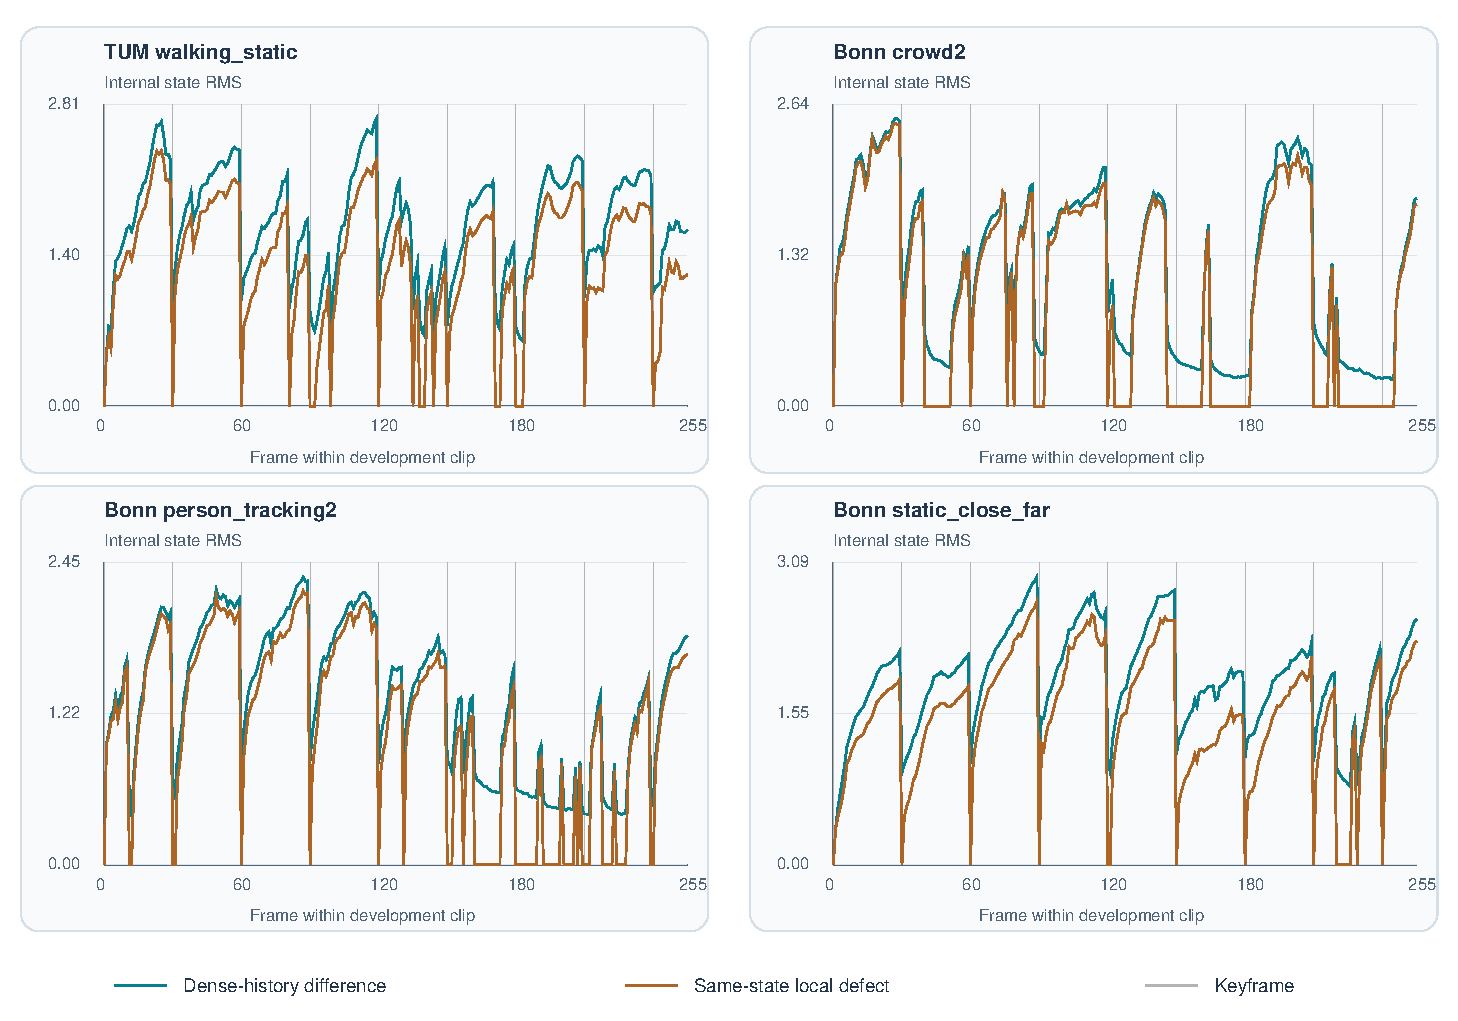
\includegraphics[width=\linewidth]{figures/development_state_diagnostic.pdf}
\caption{Development-only extended-state diagnostics. Dotted lines mark keyframes. The same-state local defect vanishes at refresh, while the difference from the separately evolved dense history persists. Curves are RMS over concatenated hidden states and caches, not GT depth error or uniquely allocated memory.}\label{fig:diagnostic}
\end{figure}

\subsection{Model-component ablations}
Table~\ref{tab:modelablations} restores the existing development ablations to the
main model narrative. All seven conditions replay the reference K30 post-fallback
mask on the same 13 L256 clips (3328 frames); mean activity is 24.18\%.
Scores are source pixel-pooled within TUM/Bonn, then source-balanced, using one
disparity scale--shift fit per clip. Invalid fits remain included.
These are inference interventions with one checkpoint, not separately optimized
or retrained competing architectures.
\begin{table}[H]
\caption{Development-only model ablations under a shared mask. Lower AbsRel/TCE is better.
GMAC counts executed Linear/Conv2d operations only, excluding selective scan and other
operations; it is not total FLOPs or latency.}\label{tab:modelablations}
\centering\small
\begin{tabular}{lrrrr}\toprule
Configuration & AbsRel & TCE & Failed clips & Partial GMAC\\
\midrule
Both caches (reference replay) & 0.2091 & 0.0435 & 2/13 & 0.656\\
Retained-state readout + spatial cache & 0.2079 & 0.0441 & 2/13 & 0.804\\
Token-drop readout + spatial cache & 0.2317 & 0.0538 & 3/13 & 0.804\\
Retained-state readout, no output caches & 0.1863 & 0.0288 & 0/13 & 1.395\\
Token-drop readout, no spatial cache & 0.3207 & 0.0511 & 0/13 & 1.395\\
Temporal cache only & 0.1937 & 0.0275 & 0/13 & 1.247\\
Stateless predictor + output hold & 0.1953 & 0.0312 & 0/13 & 0.990\\
\bottomrule\end{tabular}
\end{table}
With spatial caching enabled and temporal caching disabled, retained-state readout
has lower AbsRel and TCE than zeroing its inactive temporal residual contribution.
This supports the role of readout under that intervention, not universal superiority
over token-dropping systems. Removing spatial caching improves these depth scores
while increasing counted work. The simple output-hold control also improves these
scores over reference replay. Consequently, the present dual-cache configuration
is a particular quality--reuse trade-off, not a demonstrated optimum. We omit the
older ablation latency here because its timing subset and boundary differ from
the complete accuracy evaluation and from the main PNG-to-depth measurements.

\subsection{Post-hoc scale-variation diagnostic}
To address the earlier self-review, we summarize statistics already stored during final evaluation. This analysis was added after test access, not preregistered as a primary endpoint. It includes all eight frozen models and both lengths without tuning or new inference. For each valid frame, $s_t=\operatorname{median}(G_t)/\operatorname{median}(D_t)$ uses the same GT-valid pixels. We report the within-clip sample coefficient of variation $\operatorname{sd}(s_t)/\overline{s}$, sample standard deviation of $\log s_t$, and mean absolute log difference between consecutive retained valid frames. The scorer skips frames without valid GT and returns zero if fewer than two remain; these conventions are unchanged. Native models use no-fit depth; relative models use their median-gauge inverse-disparity depth, not an affine-fit depth. Away from numerical clamp activation, a positive constant clip scaling cancels from these statistics; an affine disparity shift does not. The stored scorer clamps the predicted median at $10^{-6}$, the scale factor at $10^{-12}$ and the CV denominator at $10^{-6}$.
\begin{table}[H]
\caption{Post-hoc scale statistics: clip means within each sequence, then four-sequence means. The CV interval enumerates sequence-bootstrap resamples; it is exploratory and unadjusted. Full intervals and gauge/failure counts are supplied as CSV.}\label{tab:scale}
\centering\small
\begin{tabular}{lrrrrr}\toprule
Model & CV L8 & CV L256 & L256 CV interval & Log-SD & Log-step \\
\midrule
Sparse K30 & 0.0312 & 0.2185 & [0.0770, 0.3601] & 0.1800 & 0.0180 \\
Sparse K5 & 0.0318 & 0.2131 & [0.0677, 0.3585] & 0.1752 & 0.0183 \\
Dense carry & 0.0312 & 0.2101 & [0.0642, 0.3560] & 0.1723 & 0.0169 \\
Dense reset & 0.0355 & 0.2463 & [0.0677, 0.4248] & 0.1903 & 0.0235 \\
Output hold & 0.0338 & 0.2466 & [0.0683, 0.4250] & 0.1905 & 0.0218 \\
DA2 Small 252 & 0.0744 & 0.2477 & [0.1753, 0.3201] & 0.2418 & 0.0696 \\
MiDaS Small 256 & 0.0603 & 0.1892 & [0.1104, 0.2680] & 0.1760 & 0.0559 \\
DPT-Large 256 & 0.0774 & 0.2554 & [0.1613, 0.3496] & 0.2219 & 0.0704 \\
\bottomrule\end{tabular}
\end{table}
A smaller scale statistic alone does not establish better depth, and per-frame fitting can hide scale errors that a metric deployment still incurs. L8 and L256 use partly different footage and reset schedules, so their difference is not an isolated causal effect of history length. Local shape changes can also affect the scale medians. These summaries are not an additive decomposition of AbsRel into scale and shape terms. Confidence intervals containing a null difference do not establish equivalence.

\begin{figure}[H]
\begin{adjustwidth}{-\extralength}{0cm}
\centering
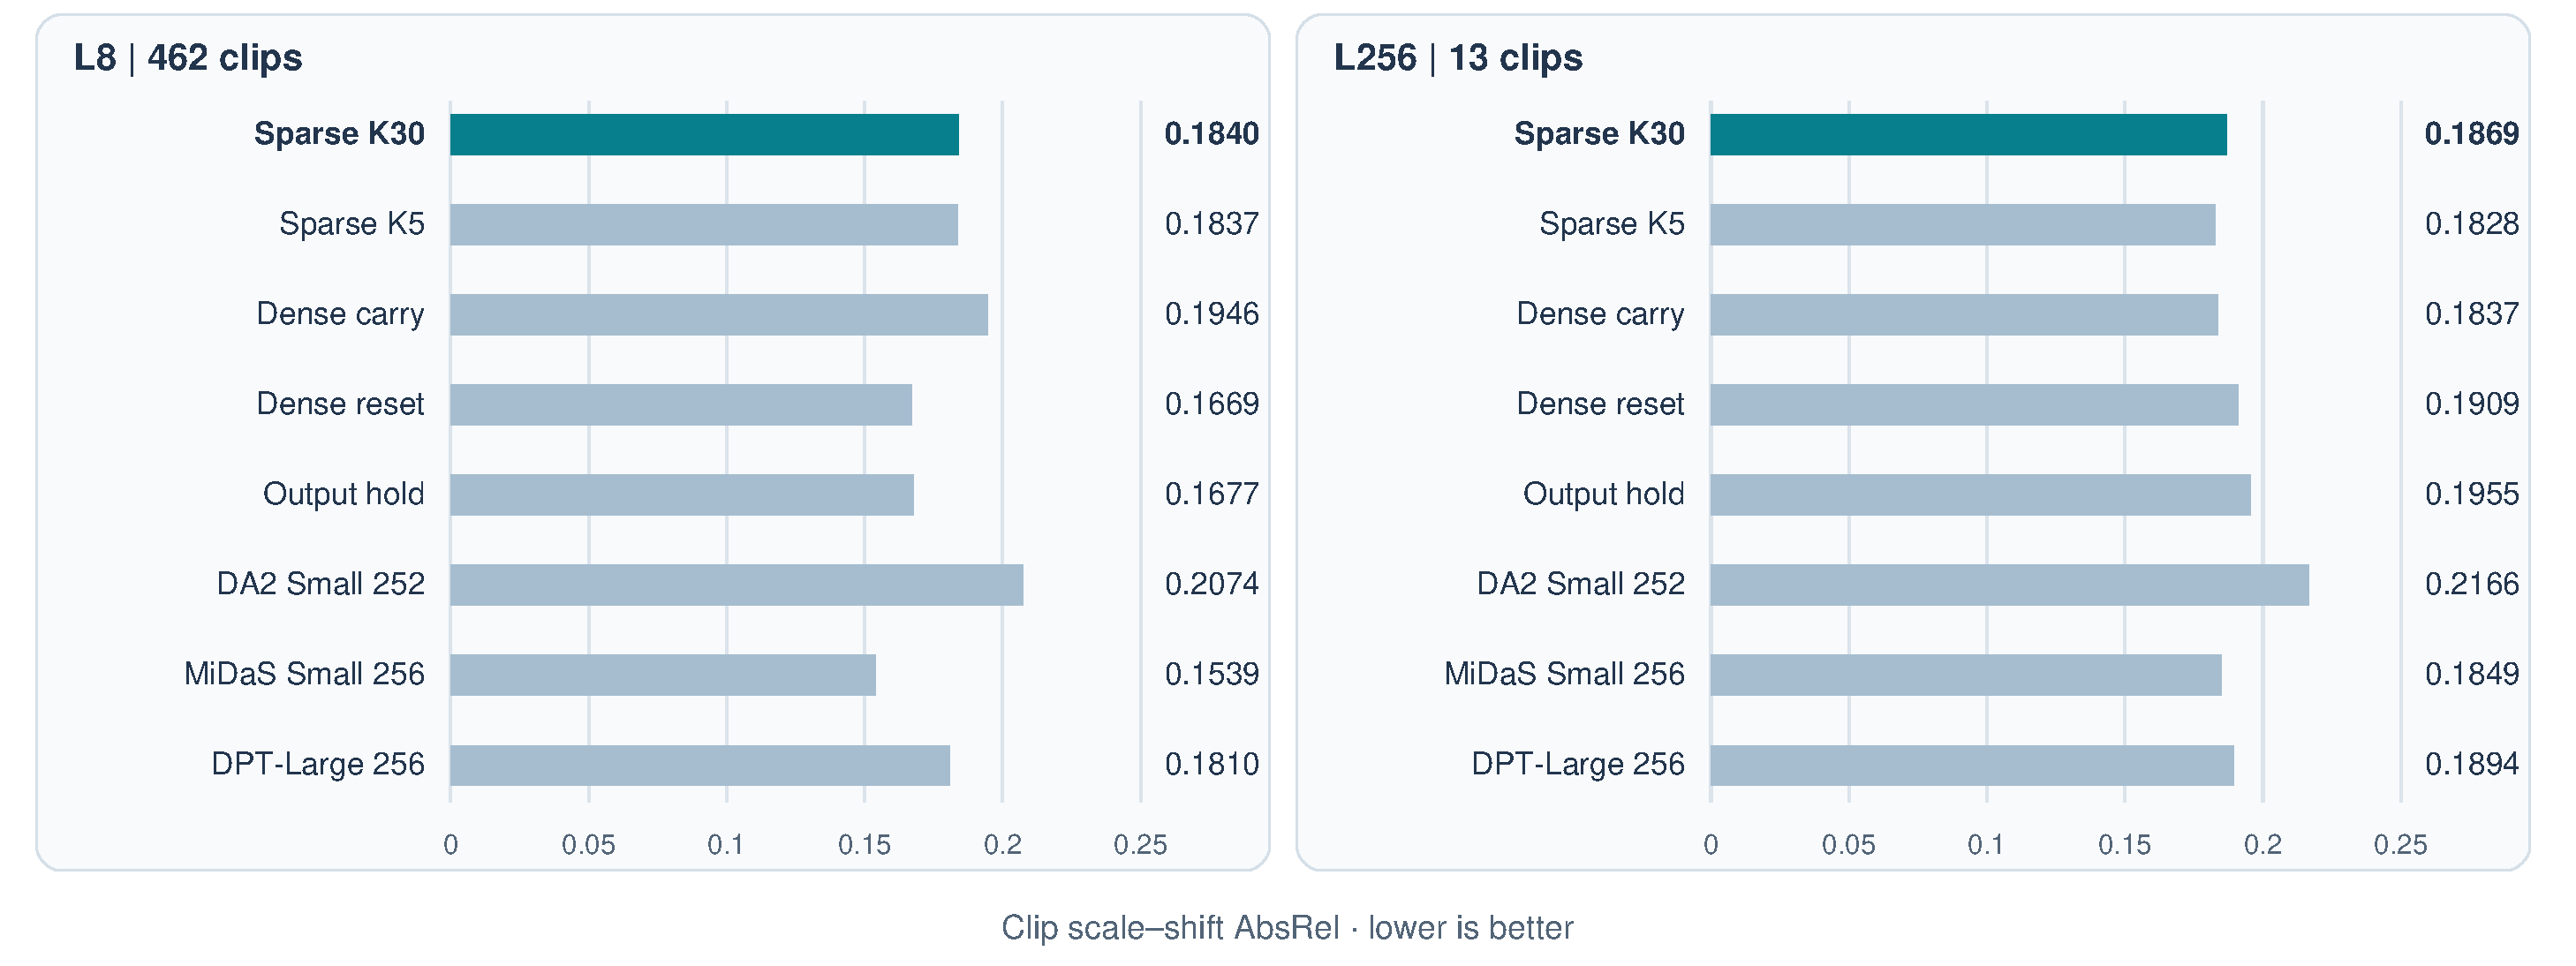
\includegraphics[width=\fulllength]{figures/r3_accuracy.pdf}
\caption{All eight frozen paths on L8 and L256, using the source pixel-pooled
clip scale--shift AbsRel estimator of the main tables. Zero-based axes and all
failed fits are retained. These point estimates have no sequence uncertainty
bars: the exploratory paired sequence estimator is reported separately.
The two lengths share some footage but are not identical history interventions.}\label{fig:accuracy}
\end{adjustwidth}
\end{figure}

\begin{figure}[H]
\begin{adjustwidth}{-\extralength}{0cm}
\centering
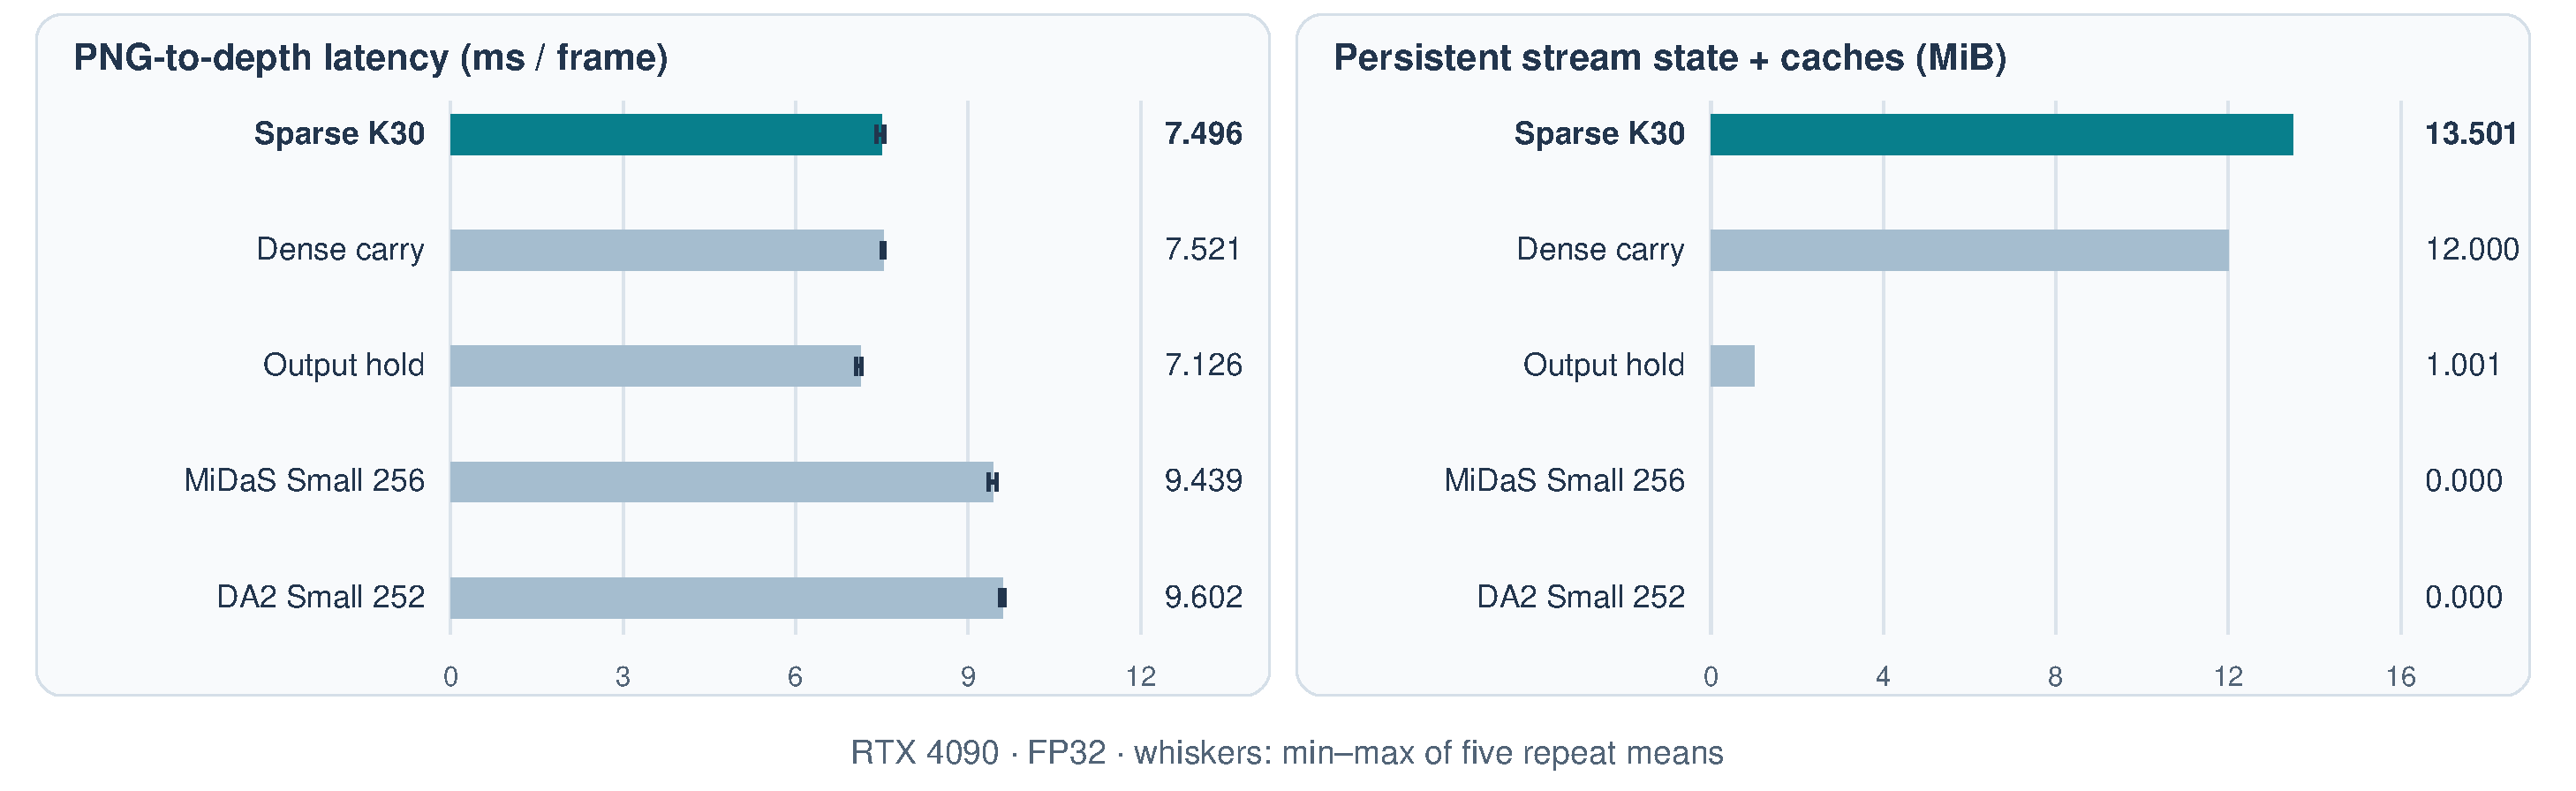
\includegraphics[width=\fulllength]{figures/r3_cost.pdf}
\caption{Development-only measured cost for five representative operating points.
Latency includes the same PNG-to-depth boundary on four matched L256 clips;
whiskers show the minimum/maximum of five repeat means, not confidence intervals.
Persistent stream memory excludes weights and transient buffers; zero state in
an image model does not mean zero total memory. Final-test accuracy is not used
to claim matched-quality acceleration.}\label{fig:cost}
\end{adjustwidth}
\end{figure}

\begin{figure}[H]
\begin{adjustwidth}{-\extralength}{0cm}
\centering
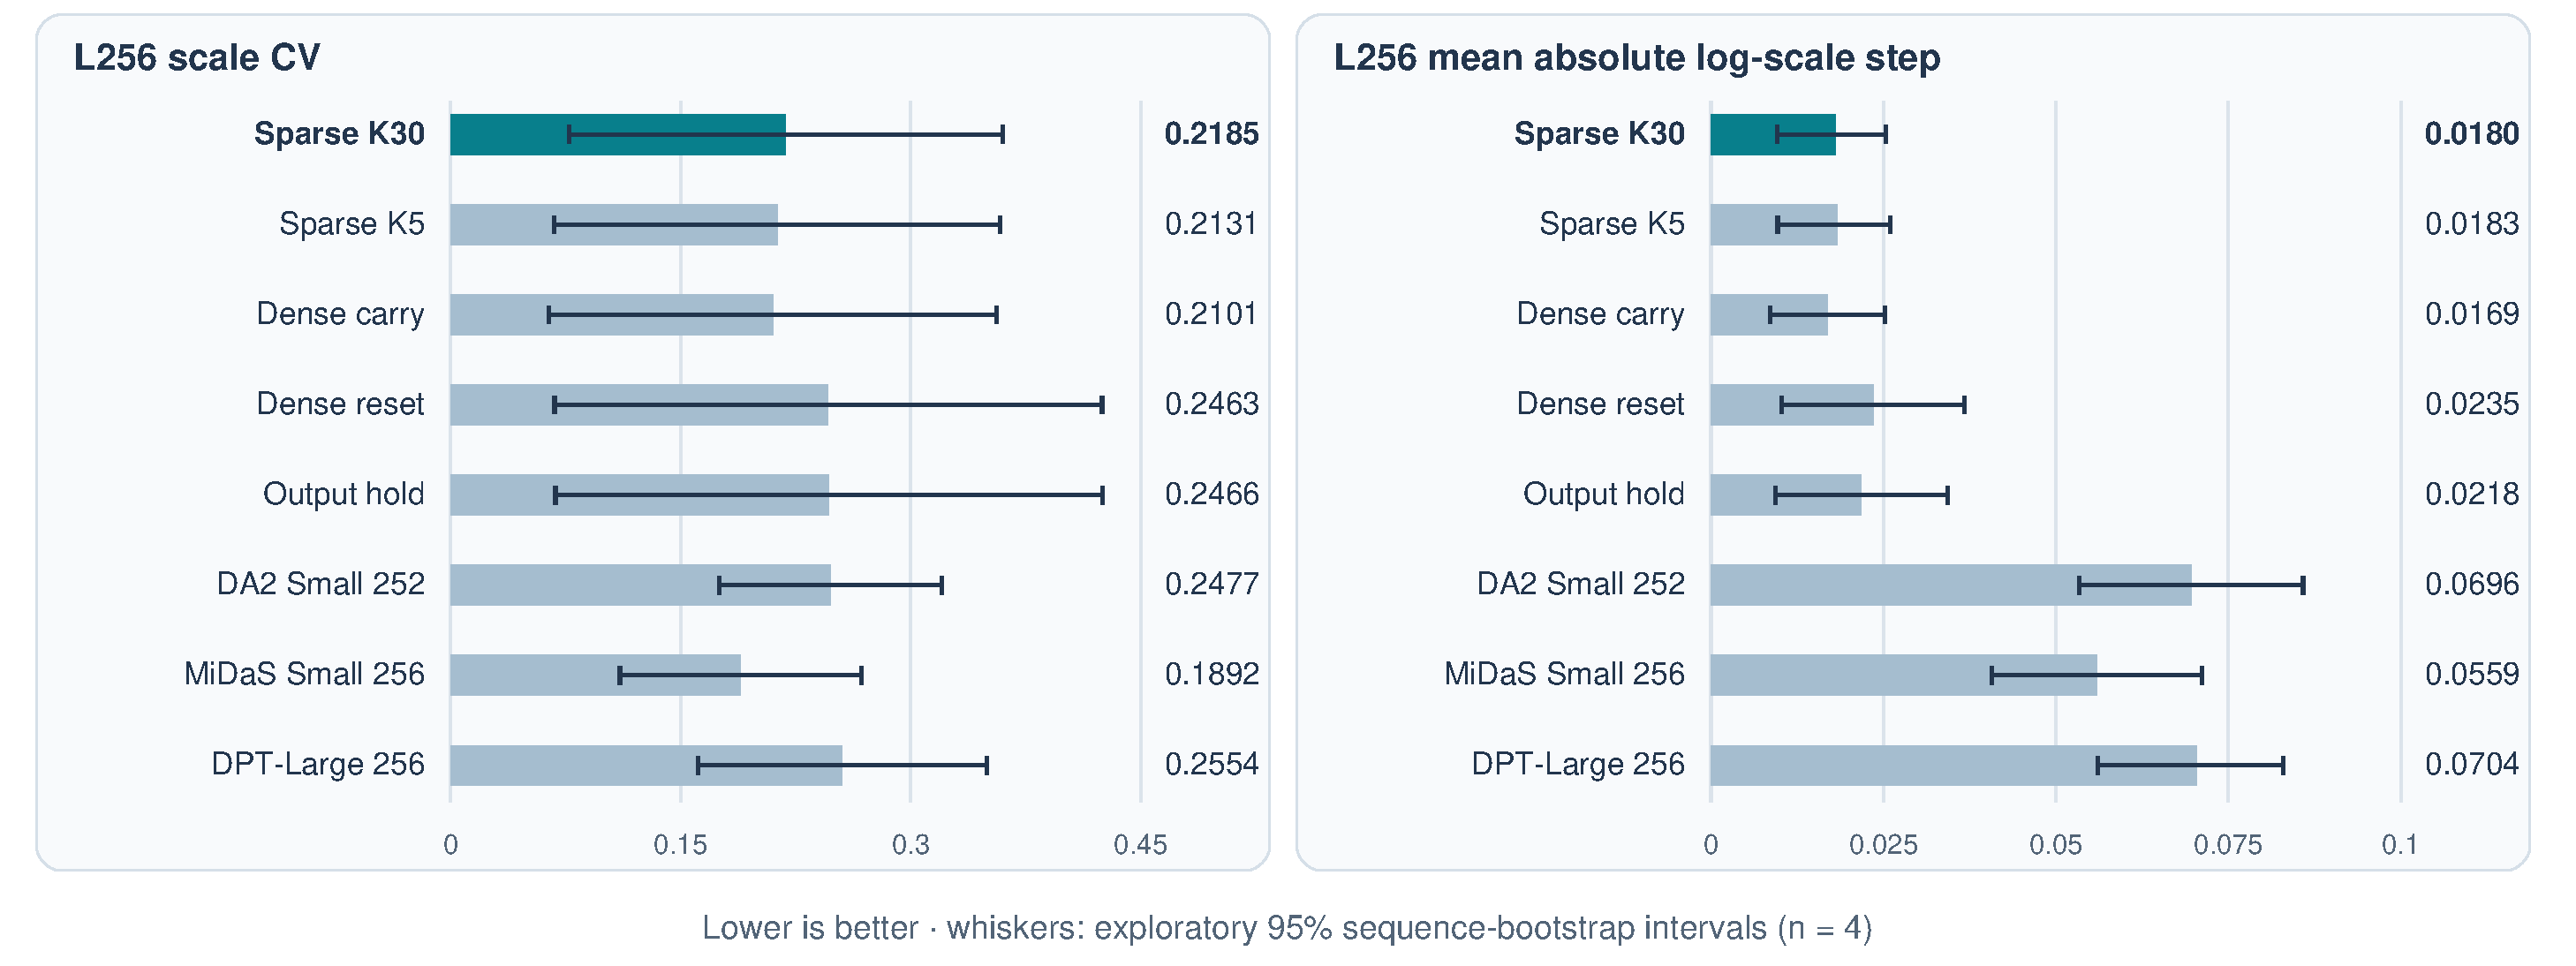
\includegraphics[width=\fulllength]{figures/r3_scale.pdf}
\caption{Post-hoc scale diagnostics for all eight frozen L256 paths. Four-sequence
means and exploratory, unadjusted percentile sequence-bootstrap intervals;
clip means are averaged within each sequence first. Native predictions use
no-fit depth, while relative predictions use median-gauge depth. CV describes
within-clip variation and log-step describes short-step variation; neither is
a substitute for depth accuracy or proof of general temporal superiority.}\label{fig:scale}
\end{adjustwidth}
\end{figure}


\subsection{Qualitative depth and temporal behavior}
Figures~\ref{fig:qualspatial} and~\ref{fig:qualtemporal} add post-hoc visualization
of the already-opened evaluation, not a new independent test. Before generating
these maps, we fixed the first L256 manifest clip of each of the four TUM
sequences (IDs tum:0, tum:4, tum:7 and tum:10), spatial frame 127, and temporal
frames 28--32 of tum:7. All frame indices are zero-based. We replayed SOKKANAEM,
dense carry, MiDaS Small and output hold from each clip boundary; all 16 complete
raw-prediction checksums exactly match the corresponding frozen results.
No weights, thresholds or aggregate scores were changed.

For visual comparability, each model uses the existing single disparity
scale--shift fit over the whole clip. This GT-assisted alignment can use later
frames and is an evaluation-only operation, not a causal inference component or
calibration-free metric output. All maps share the fixed 0--5\,m display range;
gray GT pixels are invalid, and values above 5\,m saturate without being removed
from the stored predictions or scores. No per-frame fitting or color rescaling
is used. Full input paths, alignment coefficients, invalid-fit flags, framewise
display clipping fractions and prediction hashes are supplied in
\texttt{qualitative/provenance.json}.

\begin{figure}[H]
\begin{adjustwidth}{-\extralength}{0cm}
\centering
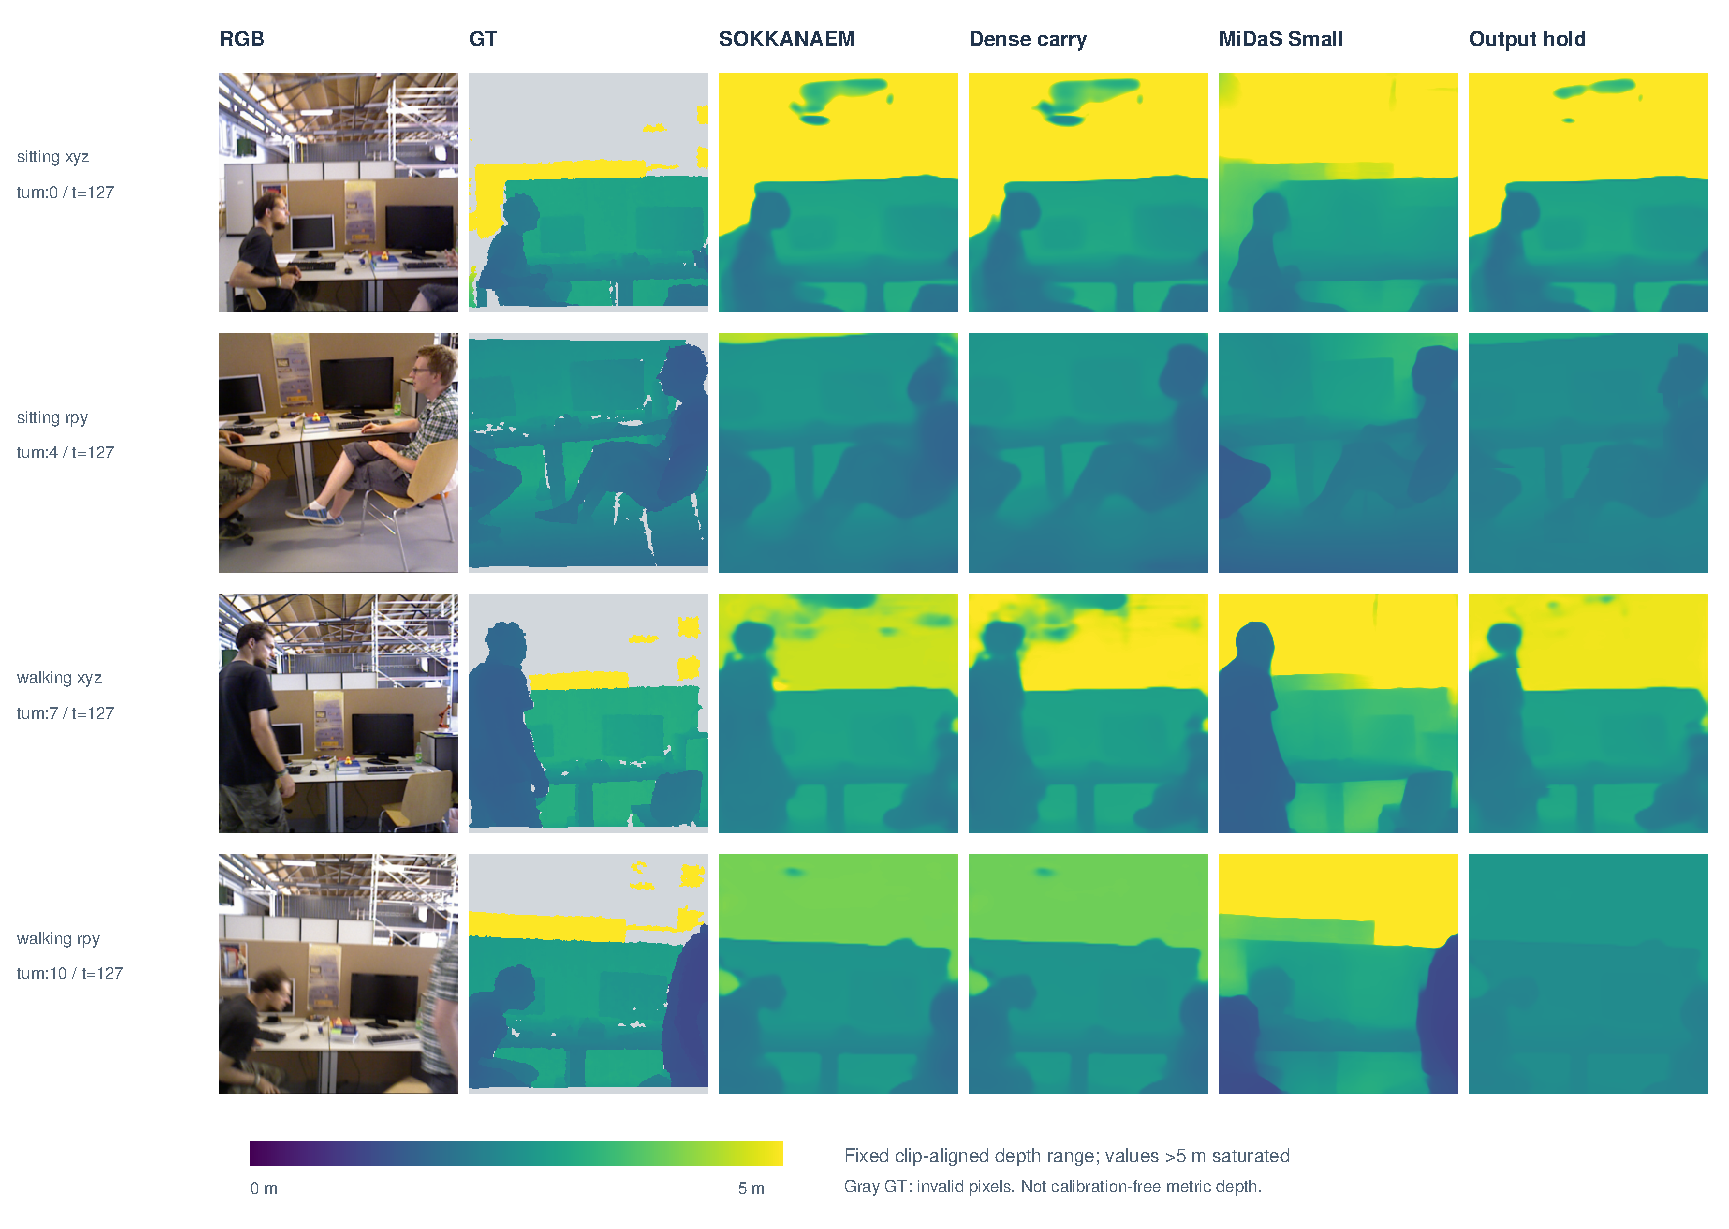
\includegraphics[width=\fulllength]{figures/qualitative_spatial.pdf}
\caption{Post-hoc qualitative comparison at fixed frame 127 of the first L256
clip in each evaluated TUM sequence. Columns show RGB, valid GT, SOKKANAEM,
dense carry, MiDaS Small and output hold. All models use one GT-assisted
disparity scale--shift fit per clip and a common fixed 0--5\,m color range.
Gray GT regions are unobserved, not zero-depth targets; saturated backgrounds
cannot establish agreement beyond the display range. The rows are fixed by
manifest order rather than selected for favorable model appearance.}
\label{fig:qualspatial}
\end{adjustwidth}
\end{figure}

The spatial examples show similar large-scale layouts for SOKKANAEM and dense
carry, but smooth outputs can suppress fine structures and person boundaries.
MiDaS preserves a more distinct foreground silhouette in the walking-xyz
example, whereas the native paths contain rounded artifacts in the distant
background. On these displayed walking-xyz and walking-rpy frames,
SOKKANAEM/MiDaS valid-GT AbsRel is respectively 0.2105/0.1196 and
0.2859/0.2028. The two sitting examples have the reverse ordering
(0.0614/0.1309 and 0.0978/0.1087). These are illustrative single-frame values,
not an additional aggregate benchmark. The selection includes tum:10, the
highest original K30 clip AbsRel among the 13 final L256 clips, so the visual
record does not exclude that adverse case. Predicted detail in invalid-GT
regions cannot be validated from these images.

\begin{figure}[H]
\begin{adjustwidth}{-\extralength}{0cm}
\centering
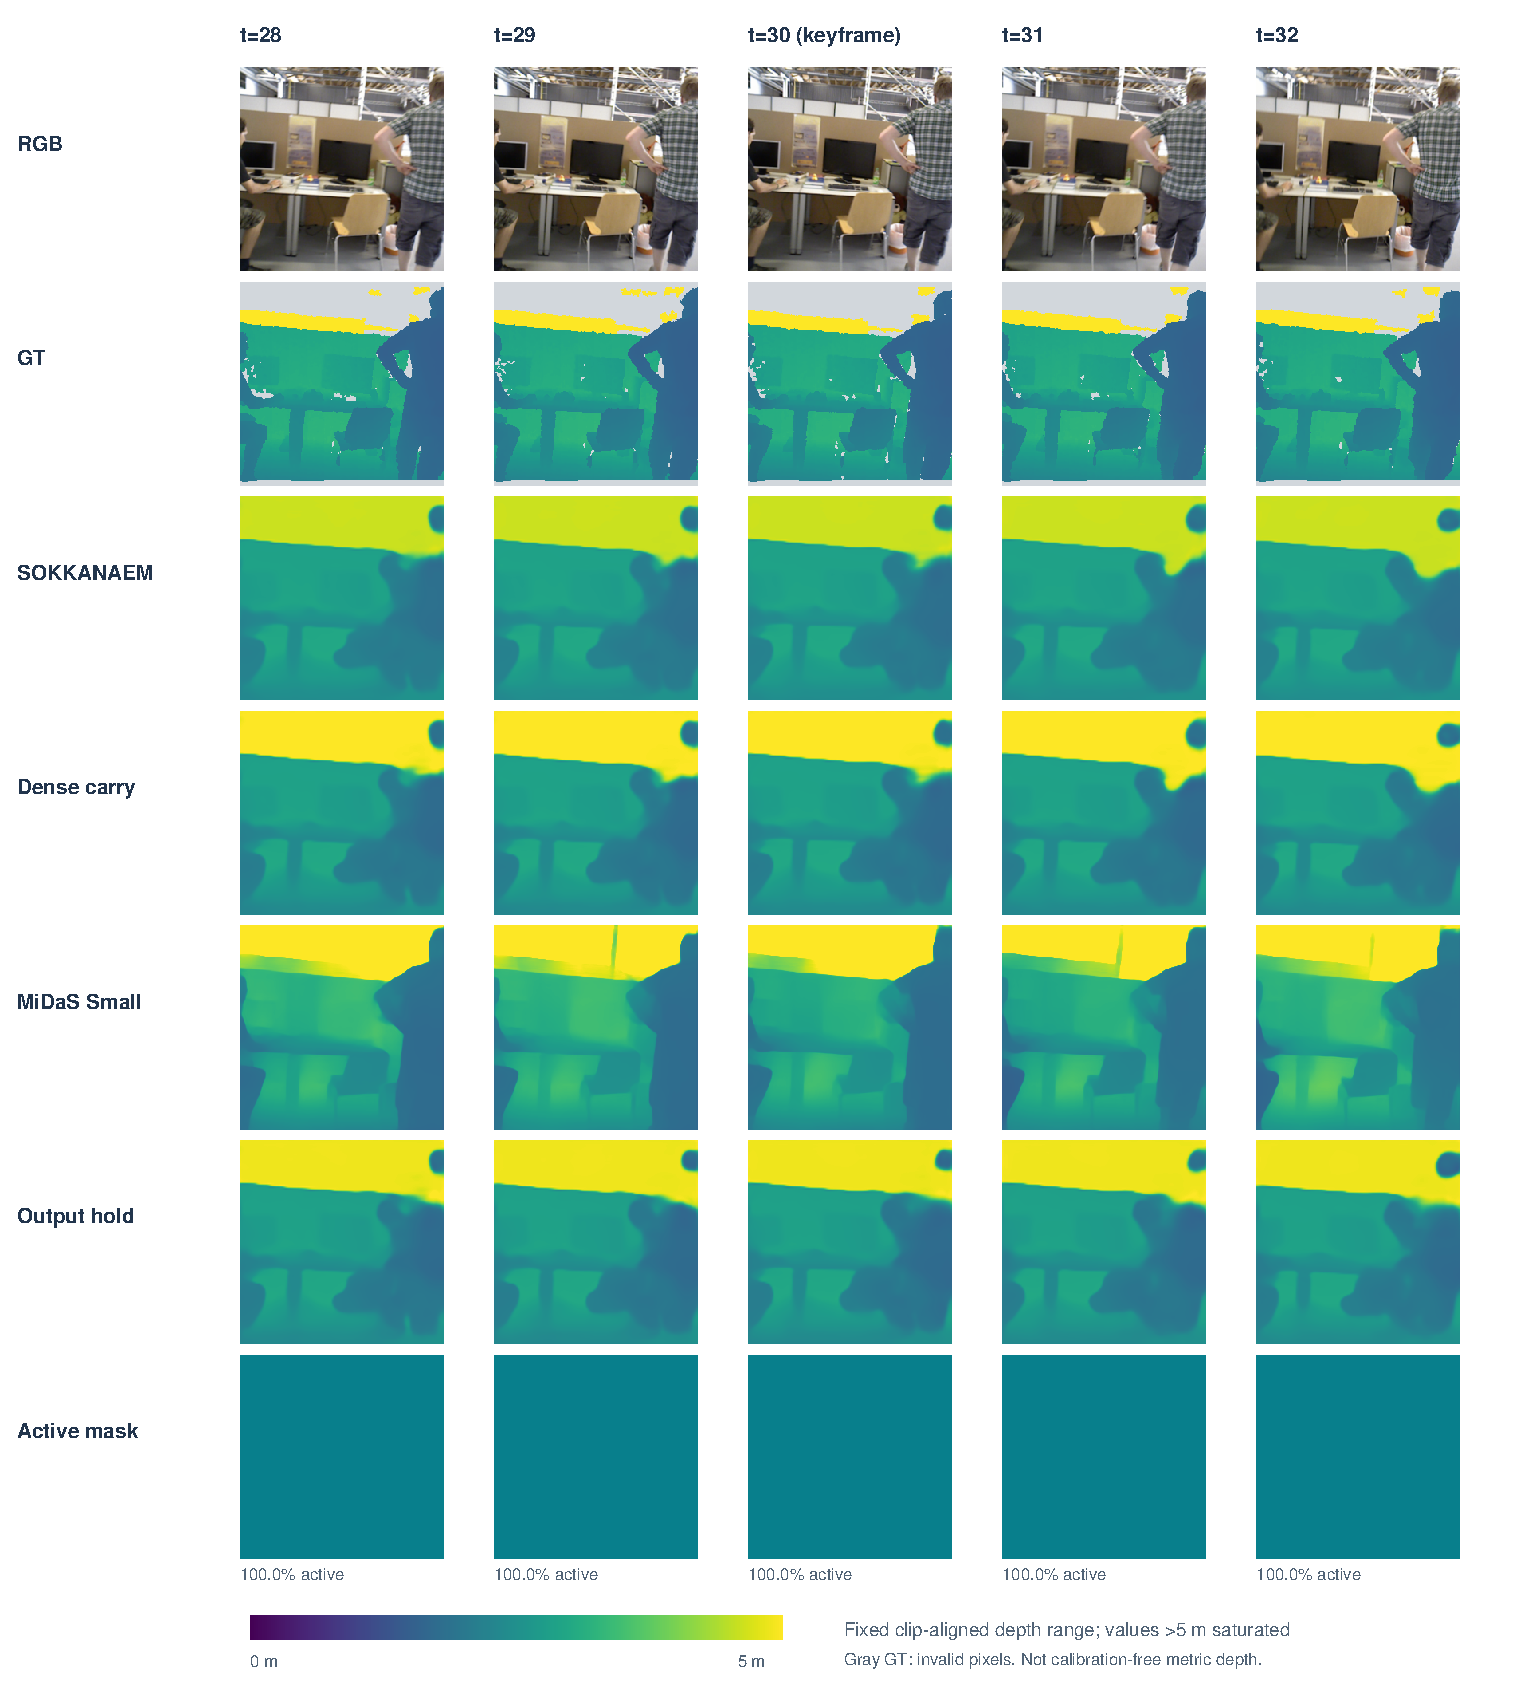
\includegraphics[width=0.86\fulllength]{figures/qualitative_temporal.pdf}
\caption{Five consecutive frames of the fixed walking-xyz clip tum:7 around
scheduled keyframe 30, with the actual post-fallback SOKKANAEM activation mask
(teal: active). All five masks are fully active, including the surrounding
non-keyframes. Thus, this example documents high-activity execution and moving
foreground boundaries; it does not isolate a sparse-reuse benefit or a causal
keyframe effect. Depth alignment, invalid-GT handling and fixed display range
are identical to Figure~\ref{fig:qualspatial}.}
\label{fig:qualtemporal}
\end{adjustwidth}
\end{figure}

In the temporal window, the native paths remain visually similar while the
moving person's outline is smoother than in the MiDaS maps. Because all five
native masks are fully active, temporal similarity here must not be attributed
to skipped updates. The supplement contains synchronized 256-frame videos for
all four selected clips (\texttt{qualitative/tum\_0.mp4},
\texttt{tum\_4.mp4}, \texttt{tum\_7.mp4}, \texttt{tum\_10.mp4}).
Playback is 10 frames/s for inspection, not measured inference throughput or
the source capture rate. These visualizations complement, rather than replace,
the quantitative temporal and accuracy measures. They do not establish general
temporal superiority or performance beyond L256.

\section{Discussion and Limitations}
The central distinction is between preservation and approximation. A constant input can
leave an ungated SSM approaching equilibrium while a skipped state remains frozen.
Similarly, recomputing every cache entry on a keyframe does not erase the history carried
by temporal states. Local defect elimination and global trajectory synchronization
are different operations, as the development diagnostic demonstrates.

The shared-input bound is useful for identifying omitted innovations, but an observed
small shadow-model residual does not certify the complete FP32 depth network. The
pixel threshold does not control all deeper features, and the spatial subsequence path
omits context even at active coordinates. Global Lipschitz constants have not been
certified. Synthetic checks and this internal derivation audit do not replace mathematical
review by the authors and an independent domain expert.

The external efficiency comparison also cannot isolate architecture from training.
MiDaS Small and DA2 Small are larger than the native network, and we have not covered
all similarly sized CNNs or modern causal video baselines. The present study supports
bounded, implementation-specific statements rather than broad accuracy or efficiency
superiority. More independent scenes and full-training replicates would be needed for
stronger generalization and stability conclusions. Test access was a one-time finalization
stage; any subsequent development would require a new untouched evaluation set.
Our 1024 development diagnostic frames comprise four separate L256 clips, not
one continuous L1024 trajectory. The older L1024 evidence concerns v9/v10,
not the present v11; its PointOdyssey aggregate scores and frame curves use
20 and 8 clips, respectively. Nearly equal endpoints cannot establish stability
throughout a trajectory. We therefore do not inherit the earlier continuous-stream
or scale/shape decomposition claims. The added current-checkpoint qualitative
replays cover four L256 clips; longer continuous evaluation remains outstanding.

\section{Conclusions}
SOKKANAEM combines patch-change selection, recurrent selective SSMs, cached block
outputs and dense decoding in a compact streaming depth model. Controlled
interventions show that retained temporal readout and spatial context influence
depth quality independently of update activity. The evaluated model offers a
specific accuracy--temporal-behavior operating point, but its current desktop
pipeline does not establish substantial sparse acceleration and its long-clip
scale variation remains a weakness. Conditional state/cache analysis explains
why refresh and computational reuse require separate quality and cost checks.
The next model-development priorities are reducing paid pipeline overhead and
controlling stale-state/cache effects without sacrificing depth accuracy; their
benefits remain to be established on an untouched evaluation set.

\supplementary{The accompanying package contains complete per-model/per-sequence tables,
frame-level development diagnostics, derivations, source hashes and reproduction commands.
Raw third-party datasets and baseline weights are obtained from their original providers.}
\authorcontributions{AUTHOR TO COMPLETE: actual contributions and approval by every author.}
\funding{AUTHOR TO COMPLETE: funding sources and grant identifiers, or a verified no-funding statement.}
\institutionalreview{AUTHOR TO CONFIRM: applicability of institutional review and dataset-use permissions.}
\informedconsent{AUTHOR TO CONFIRM: applicability of consent requirements for the reused datasets.}
\dataavailability{Derived results, code and manifest hashes are included in the local reproducibility
package. Public repository URL/DOI and redistribution permissions must be supplied and confirmed
by the authors before submission. Original TUM/Bonn data and external weights remain subject to
their providers' terms.}
\acknowledgments{AI assistance was used for code development, experiment orchestration,
mathematical drafting, analysis and manuscript preparation. The authors must supply tool/version
details, review and edit all outputs, and confirm responsibility before submission. This working
draft does not assert that such author review has already occurred.}
\conflictsofinterest{AUTHOR TO COMPLETE: actual competing interests or a verified absence thereof.}

\appendixtitles{yes}
\appendixstart
\appendix
\section{Analytic Proofs}\label{app:proofs}
\input{theory_appendix.tex}
\section{Reproduction Details and Evidence Boundaries}\label{app:repro}
\subsection{Checkpoint, training record and interventions}
The archived effective configuration beside the seed-0 v11 checkpoint records
8000 final-stage steps, clip length 24, batch size 2, image size 256, learning
rate $3\times10^{-4}$, 1000 warmup steps, gradient-norm clipping at 1 and EMA
decay 0.999. The checkpoint resumes partially from v10. The recorded loss
weights are multiscale gradient 0.5, normal 0.05, warp 2, spread 0.5, edge 2,
and bin classification 0.2. Teacher and feature-distillation weights are zero
in this stage only. Training uses random masks with maximum skip fraction 0.5;
the image-change detector is not used to generate these training masks.

The archived training implementation uses AdamW (default weight decay 0.01),
warmup followed by cosine learning-rate decay, and source-balanced weighted
sampling over TUM, Bonn, VKITTI2, TartanAir2 and PointOdyssey. Clip-consistent
augmentation comprises zoom/crop with scale 0.55--1.0, horizontal flip with
probability 0.5, brightness/contrast factors 0.75--1.3, saturation 0.7--1.4,
and gamma 0.8--1.25. The effective v11
sidecar records augmentation enabled and the dataset paths, but not all of
these sampler/optimizer implementation details or the RNG trajectory.
These are reproduction settings read from the archived implementation, not
an independently reconstructed historical run. The sidecar's recorded source
commit is \texttt{0a3f5e06abbf448898a65c0a42c53534531912e5}.
The four-stage ancestry, rather than the earlier three-stage summary, must be
used when describing training cost. Full-training seed variation remains unknown.

Only one reference operating configuration is selected: K30, thresholds
0.05/0.025, fallback 0.4, both caches on and GMC off. K5, dense carry, dense
reset and output hold are frozen diagnostic controls, not post-test deployment
recommendations. The development cache/readout interventions are available in
the study-5--8 tables. Historical threshold/fallback sweeps remain in the older
draft's Table 9, not a newly validated frozen-protocol sensitivity panel. None
of these should be mixed with final-test scores. A token-drop control zeroes
the inactive temporal residual contribution (retaining the identity bypass
and frozen hidden state); it is not equivalent to dropping input
video frames. No universal accuracy gain over that control is claimed.

\subsection{Temporal-score equations and masking}
Let $D_t$ be depth after the declared clip gauge and $G_t$ ground truth.
RAFT Small uses RGB mapped from $[0,1]$ to $[-1,1]$ at the common evaluation
resolution and its final refinement output, with the default pretrained
weights resolved by the frozen dependency record. Flow maps the current
frame to the preceding frame. Let $W_t$ warp that preceding frame with
nearest-neighbor sampling, border padding and aligned grid corners.
The common mask $m_t$ is the product of the in-bounds indicator, current
GT validity and warped previous GT validity. There is no forward--backward
flow-consistency or semantic occlusion filter. With $N_m=\max(1,\sum_{t,i}m_{t,i})$,
\begin{align}
 \mathrm{OPW}&=\frac{1}{N_m}\sum_{t,i}m_{t,i}
  \frac{|(W_tD_{t-1})_i-D_{t,i}|}{\max(G_{t,i},10^{-6})},\\
 \mathrm{TCE}&=\frac{1}{N_m}\sum_{t,i}m_{t,i}
  \frac{|(W_tD_{t-1})_i-D_{t,i}-(W_tG_{t-1})_i+G_{t,i}|}
       {\max(G_{t,i},10^{-6})}.
\end{align}
Both are dimensionless. Raw temporal delta is the mean absolute consecutive
depth difference over all pixels, without warping or a GT-validity mask,
after the declared clip alignment; it has depth units and is not itself a
ground-truth temporal-accuracy measure. Temporal scores are not reported after
per-frame fitting, which would change the temporal signal. All code-level
clamps and invalid-fit conventions remain those of the frozen scorer.

\subsection{Memory, edge evidence and portability}
For $N$ independent streams, persistent storage is $W+NS$, before input/output
buffers, temporary activations and allocator overhead. The native FP32 weights
occupy about 15.968 MiB; K30 state plus caches occupies 13.501 MiB per stream,
versus 12.000 MiB for dense carry without output caches. This is not peak VRAM,
and inactive states are still densely allocated. Fewer parameters or updates
therefore do not by themselves establish lower latency or multi-stream memory.

Historical Nano Developer Kit B01 logs cover user-confirmed 5 W and 10 W modes,
but use a reference scan, fixed-ratio activity and repeated synthetic inputs.
They are not the fused desktop path or the measured PNG-to-depth pipeline.
The power source is module VDD\_IN, not whole-system wall power. Missing
historical weight/code linkage and independent power repetitions prevent
those logs from establishing final-model real-video energy savings. Their
separate audit is supplied without a quantitative edge claim in this paper.

The private package includes source, derived scores, manifests, configuration
and native weights; original media and third-party baseline weights require
separate authorized acquisition. Frozen paths may need a versioned relocation
manifest on another machine. Full clean-machine training/inference reproduction
and independent human verification have not been performed. The complete
40-item internal-review response is provided separately; partial and withdrawn
items must not be read as experimentally resolved.


\reftitle{References}
\begin{thebibliography}{99}
\bibitem{vda} Chen, S.; Guo, H.; Zhu, S.; Zhang, F.; Huang, Z.; Feng, J.; Kang, B.
Video Depth Anything: Consistent Depth Estimation for Super-Long Videos. CVPR, 2025.
\url{https://arxiv.org/abs/2501.12375}.
\bibitem{ovda} Feiden, J.-F.; K\"uchler, T.; Zavadski, D.; Savchynskyy, B.; Rother, C.
Online Video Depth Anything: Temporally-Consistent Depth Prediction with Low Memory Consumption.
arXiv:2510.09182, 2025. \url{https://arxiv.org/abs/2510.09182}.
\bibitem{campos2018} Campos, V.; Jou, B.; Gir\'o-i-Nieto, X.; Torres, J.; Chang, S.-F.
Skip RNN: Learning to Skip State Updates in Recurrent Neural Networks. ICLR, 2018.
\url{https://arxiv.org/abs/1708.06834}.
\bibitem{gu2024} Gu, A.; Dao, T. Mamba: Linear-Time Sequence Modeling with Selective State Spaces.
arXiv:2312.00752v2, 2024. \url{https://arxiv.org/abs/2312.00752}.
\bibitem{deltacnn} Parger, M.; Tang, C.; Twigg, C.D.; Keskin, C.; Wang, R.; Steinberger, M.
DeltaCNN: End-to-End CNN Inference of Sparse Frame Differences in Videos. CVPR, 2022.
\url{https://arxiv.org/abs/2203.03996}.
\bibitem{eventful} Dutson, M.; Li, Y.; Gupta, M.
Eventful Transformers: Leveraging Temporal Redundancy in Vision Transformers. ICCV, 2023.
\url{https://arxiv.org/abs/2308.13494}.
\bibitem{spikessm} Zhong, Y.; Zhao, R.; Wang, C.; Guo, Q.; Zhang, J.; Lu, Z.; Leng, L.
SPikE-SSM: A Sparse, Precise, and Efficient Spiking State Space Model for Long Sequences Learning.
arXiv:2410.17268, 2024. \url{https://arxiv.org/abs/2410.17268}.
\bibitem{spikyspace} Tang, K.; Zheng, J.; Jin, Y.; Qiu, Y.; Sun, G.; Yan, Z.; Wong, W.-F.
SpikySpace: A Spiking State Space Model for Energy-Efficient Time Series Forecasting.
arXiv:2601.02411v2, 2026. \url{https://arxiv.org/abs/2601.02411}.
\bibitem{dpt} Ranftl, R.; Bochkovskiy, A.; Koltun, V.
Vision Transformers for Dense Prediction. ICCV, 2021. \url{https://arxiv.org/abs/2103.13413}.
\bibitem{midas} Ranftl, R.; Lasinger, K.; Hafner, D.; Schindler, K.; Koltun, V.
Towards Robust Monocular Depth Estimation: Mixing Datasets for Zero-shot Cross-dataset Transfer.
\url{https://arxiv.org/abs/1907.01341}.
\bibitem{da2} Yang, L.; Kang, B.; Huang, Z.; Zhao, Z.; Xu, X.; Feng, J.; Zhao, H.
Depth Anything V2. arXiv:2406.09414, 2024. \url{https://arxiv.org/abs/2406.09414}.
\bibitem{amdahl1967} Amdahl, G.M. Validity of the single processor approach to achieving
large scale computing capabilities. AFIPS Spring Joint Computer Conference, 1967, 483--485.
\url{https://doi.org/10.1145/1465482.1465560}.
\bibitem{tumdata} Sturm, J.; Engelhard, N.; Endres, F.; Burgard, W.; Cremers, D.
A Benchmark for the Evaluation of RGB-D SLAM Systems. IROS, 2012, 573--580.
\url{https://cvg.cit.tum.de/_media/spezial/bib/sturm12iros.pdf}.
\bibitem{bonndata} Palazzolo, E.; Behley, J.; Lottes, P.; Gigu\`ere, P.; Stachniss, C.
ReFusion: 3D Reconstruction in Dynamic Environments for RGB-D Cameras Exploiting Residuals.
IROS, 2019. \url{https://arxiv.org/abs/1905.02082}.
\end{thebibliography}
\end{document}
